\documentclass[9pt]{beamer-control}
\usepackage{beamer-control-workshop}
\begin{document}
\CONCEPT[1]{Week 1: Introduction and System Modelling}

\begin{SUMMARY}
\begin{itemize}
\item Matlab introduction
\item Modelling an ODE in Matlab
\item Simulink introduction
\item Modelling an ODE in Simulink
\item Save an output graph
\end{itemize}
\end{SUMMARY}


\begin{frame}
\frametitle{Introduction}
In this workshop, we will introduce the Matlab and Simulink environments and use them to build and visualise some simple dynamical systems.
\end{frame}

\SUBCONCEPT{Matlab basics}

\begin{frame}
\frametitle{Why Matlab?}
\begin{itemize}
\item Matlab started life as a mathematical programming language and has evolved into a more general programming language
\item Much development in the last 10 years to make it act and feel more modern (e.g., key=val function arguments, real strings, etc.)
\item We use Matlab for several reasons:
\begin{itemize}
\item  Industry standard in control systems
\item  Good support for control systems via (several) toolboxes -- one stop shop
\item  Simulink supports real-time hardware: this is one reason that Matlab is an industry standard -- can prototype, simulate, and deploy within Matlab/Simulink directly
\item  Very good visualisation tools
\end{itemize}
\item If you are coming from Python, the learning curve is reasonably shallow, but there are some notable differences (e.g., indexing from \texttt{1}, need to use many more semicolons)
\item If you struggle with Matlab syntax or features, Mathworks has excellent training videos
\end{itemize}
\end{frame}

\begin{frame}
\frametitle{Matlab intro}

\begin{itemize}
\item Matlab and Simulink are detailed components of this course
\item You will learn:
\begin{itemize}
\item  How to write m-files (scripts), and possibly functions, to solve problems
\item  How to use the Matlab Control Systems toolbox as a `recipe book' for control problems
\item  How to use Simulink to model and simulate dynamical systems
\end{itemize}
\item On the next page you can see how I set up my Matlab environment, with the following interfaces:
\begin{itemize}
\item Top: Ribbon bar with Editor tab and Run button
\item Second top: Working directory path -- make sure this is where your files are!
\item Left: Working directory files -- organise this, say, with a new folder per topic
\item Middle top: Matlab editor
\item Middle bottom: Matlab command window
\item Right: Workspace
\end{itemize}
\end{itemize}
\end{frame}

\begin{frame}
\frametitle{The IDE}
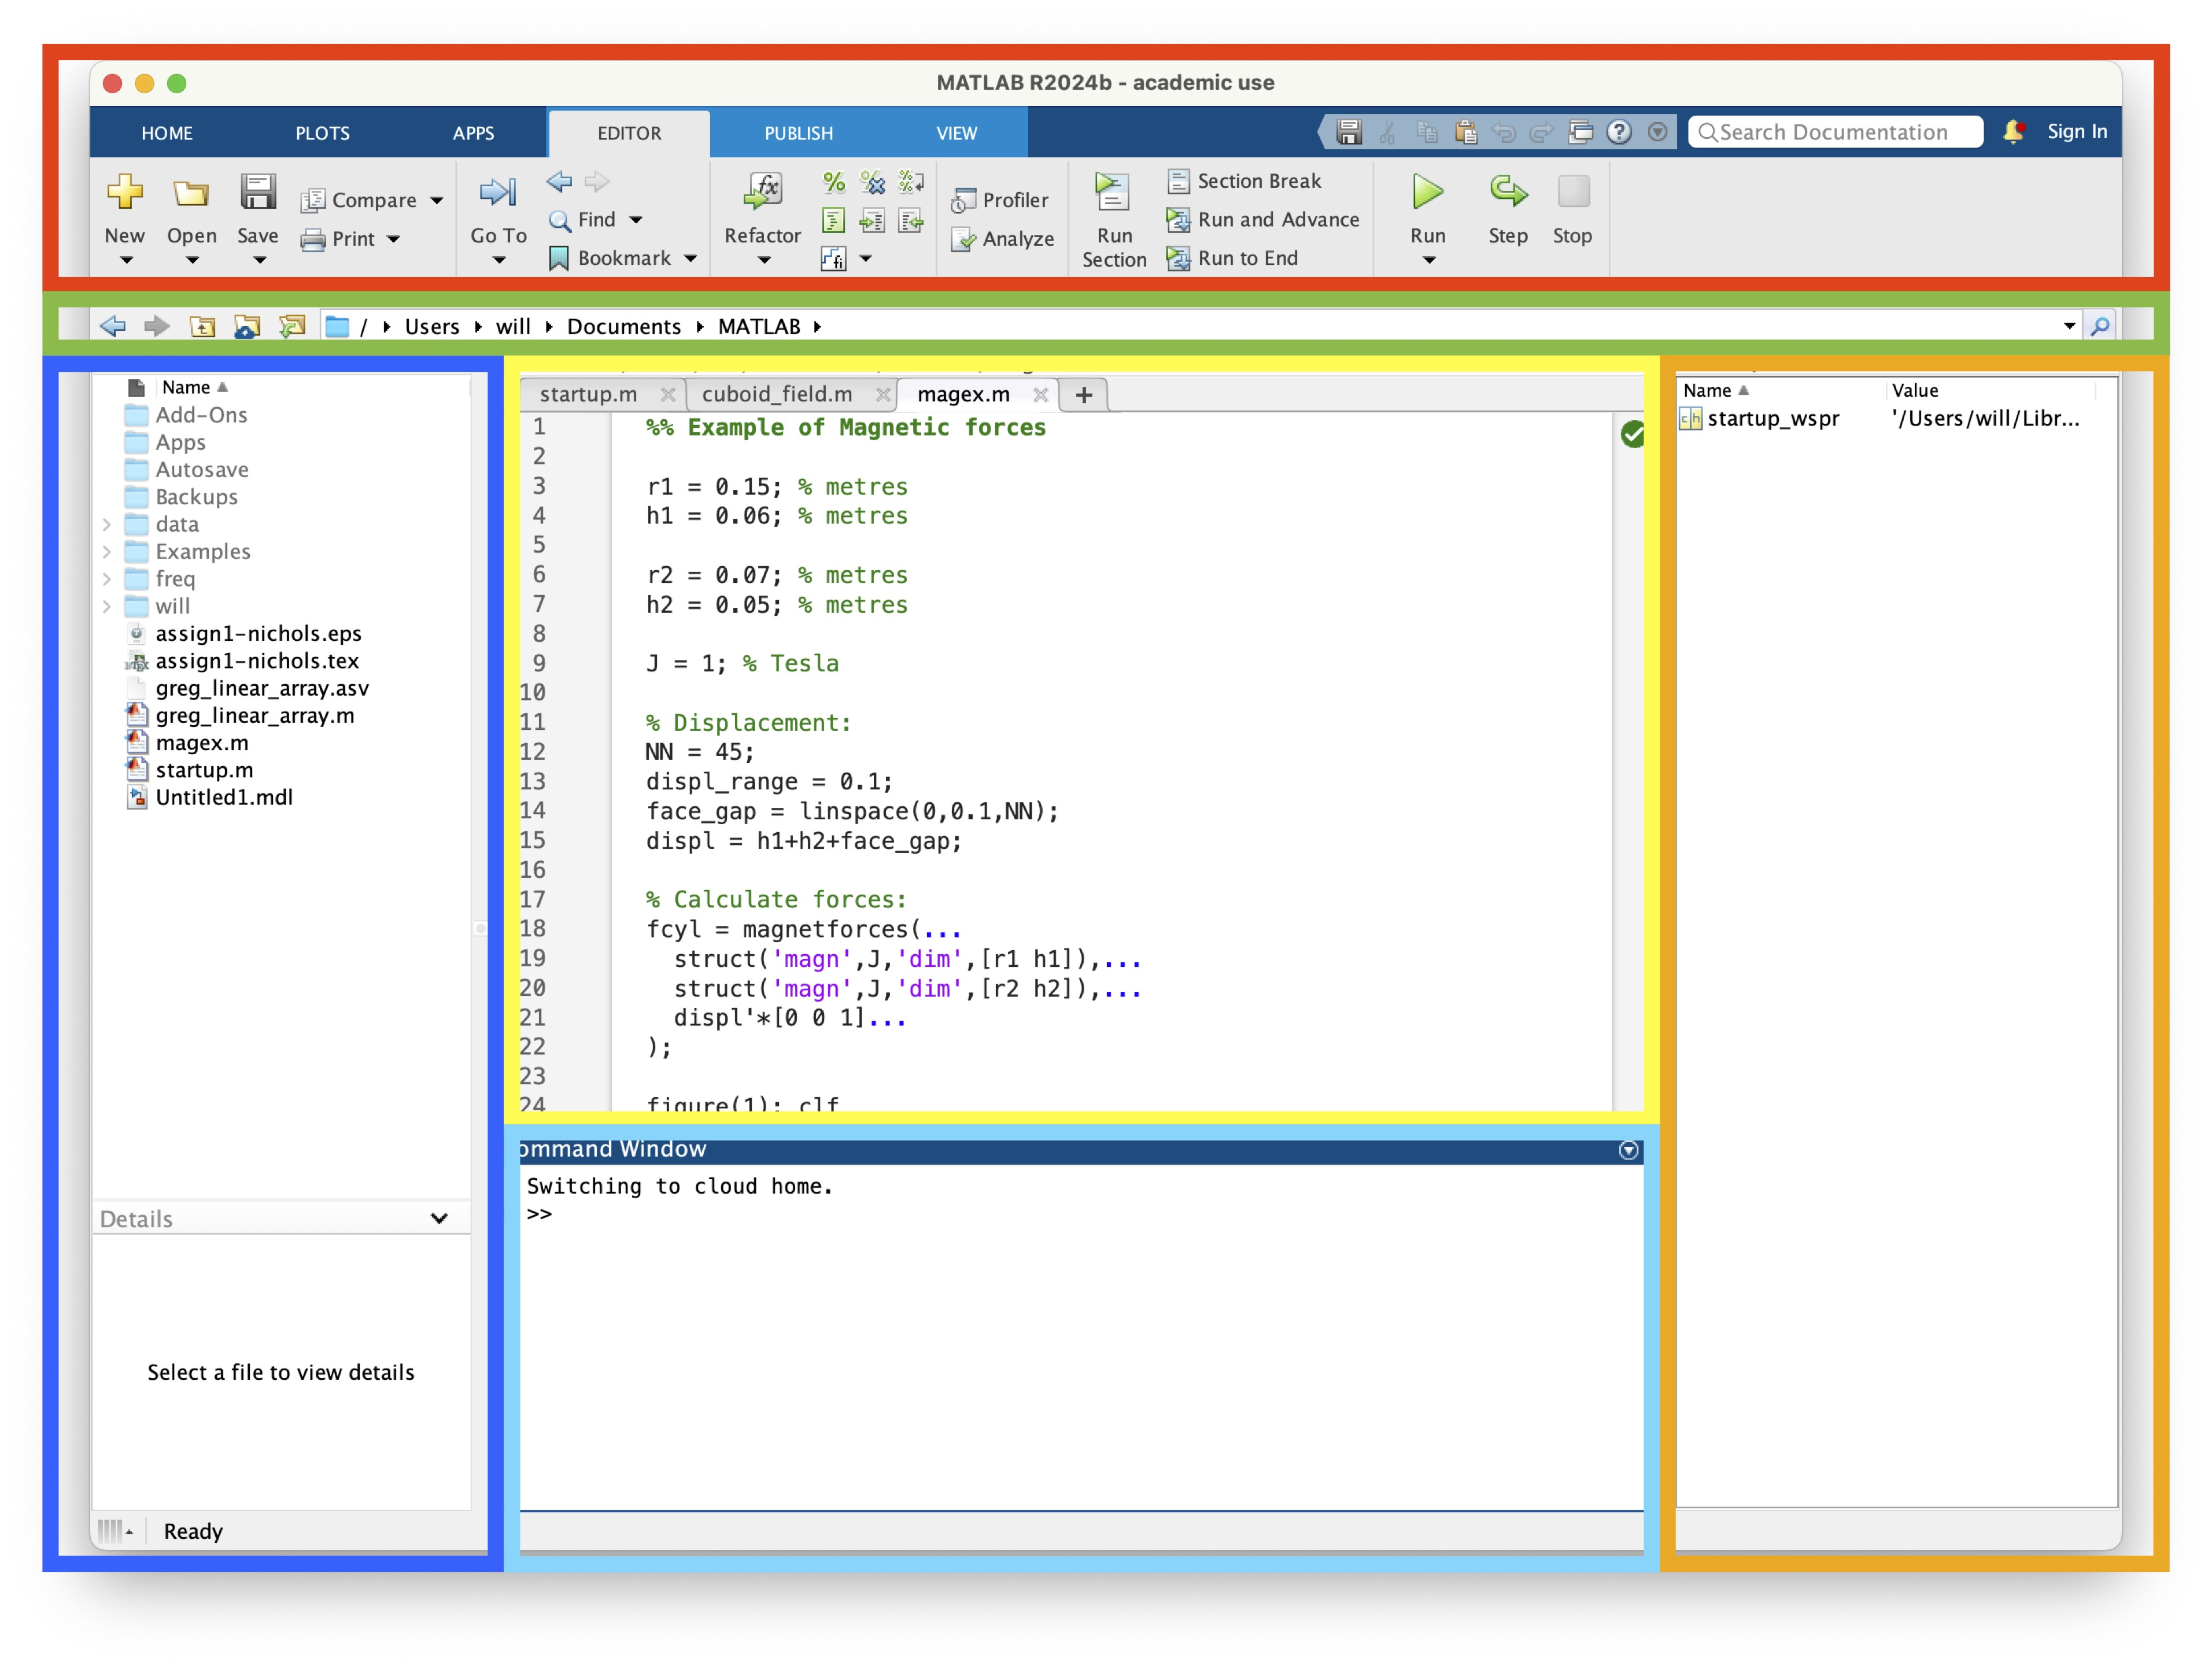
\includegraphics[width=\linewidth]{matlab-ide-annot}
\end{frame}

\begin{frame}
\frametitle{Getting starting}
\begin{enumerate}
\item Create a folder, called \CODE{Topic 1}
\item Create a file inside called \CODE{workshop1.m}\\(note, no spaces or hyphens allowed in Matlab file names)
\item Write the following:
\includematlab{workshop1.m}{part1}
\item Make sure the working directly is where the file is, and \Mbutton{Run} the file
\item What do you expect to see? Can you make the curve more smooth?
\item Now find the \Mbutton{PUBLISH} tab and \Mbutton{Publish} the file. What do you think?
\end{enumerate}
\end{frame}
\begin{frame}

\frametitle{Multiple curves}
\begin{enumerate}
\item Directly below that code, write:
\includematlab{workshop1.m}{part2}
\item Note the pattern: create a numbered figure, clear it, `hold' it, then plot
\item What happens if you don't clear it?
\item What happens if you don't hold it?
\end{enumerate}
\end{frame}

\SUBCONCEPT{ODE solving}

\begin{frame}
\frametitle{Mass-spring-damper}
\begin{itemize}
\item You may have previously solved ODEs analytically; we don't do much of that in this course
\item Consider the classical mass-spring-damper linear model:
\[
   m\ddot x + c\dot x + k x = 0
\] 
\item Copy the code to simulate this ODE shown over the page\\
 (If you are using quite an old version of Matlab, you'll need to put the function at the end of the file)
\item What are the states of this system?
\item Is acceleration a state? Why or why not?
\item Experiment with different values of $m$, $c$, $k$, and initial conditions
\item Can any of these values be negative? What happens?
\item Plot a phase diagram of this system ($\dot x$ vs $x$)
\end{itemize}
\end{frame}

\begin{frame}
\frametitle{Mass-spring-damper}
\includematlab{workshop1.m}{msd}
\end{frame}

\begin{frame}
\frametitle{Sneak peak}
\begin{itemize}
\item Let's model this system in the frequency domain instead:%
\footnote{\emph{You don't need to understand the derivation to get to this equation, but hopefully the form of the equation makes it obvious we have the same system represented differently}}
\[
  P(s) = \frac{1}{ms^2+cs+k}
\]
\item Use the code on the following slide to simulate this system. Do you see similar characteristics?
\item What is an impulse response?
\item What is a step response?
\item Which code is easier to write? Which code is more general?
\end{itemize}
\end{frame}

\begin{frame}
\frametitle{Mass-spring-damper in the frequency domain}
\includematlab{workshop1.m}{pz}
\end{frame}

\SUBCONCEPT{Simulink inputs and outputs}

\begin{frame}
\frametitle{Simulink introduction}
\begin{itemize}
\item Launch Simulink by typing \texttt{simulink} in the Command Window, or clicking New > `Simulink Model' in the GUI:
\end{itemize}
\begin{center}
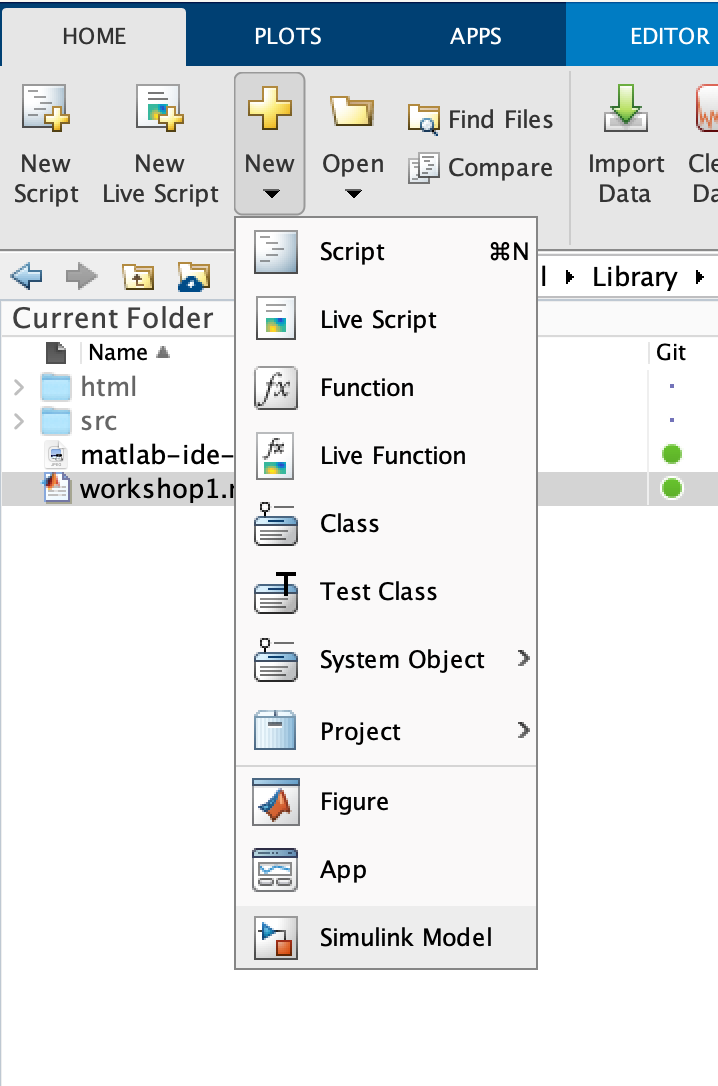
\includegraphics[height=0.5\textheight]{simulink_new_model}
\end{center}
\begin{itemize}
\item
Create and save the model with a filename like \texttt{topic1model.slx}
\end{itemize}

\end{frame}

\begin{frame}
\frametitle{Create some blocks}
\begin{itemize}
\item Double click in the empty space and type `Sine' to insert a sinusoid source
\item Double click and type 'Scope' to insert a graphing output (or `sink')
\item Click the arrows to join the source to the scope. Then click \Mbutton{Run} and double click the Scope:
\end{itemize}

\centering
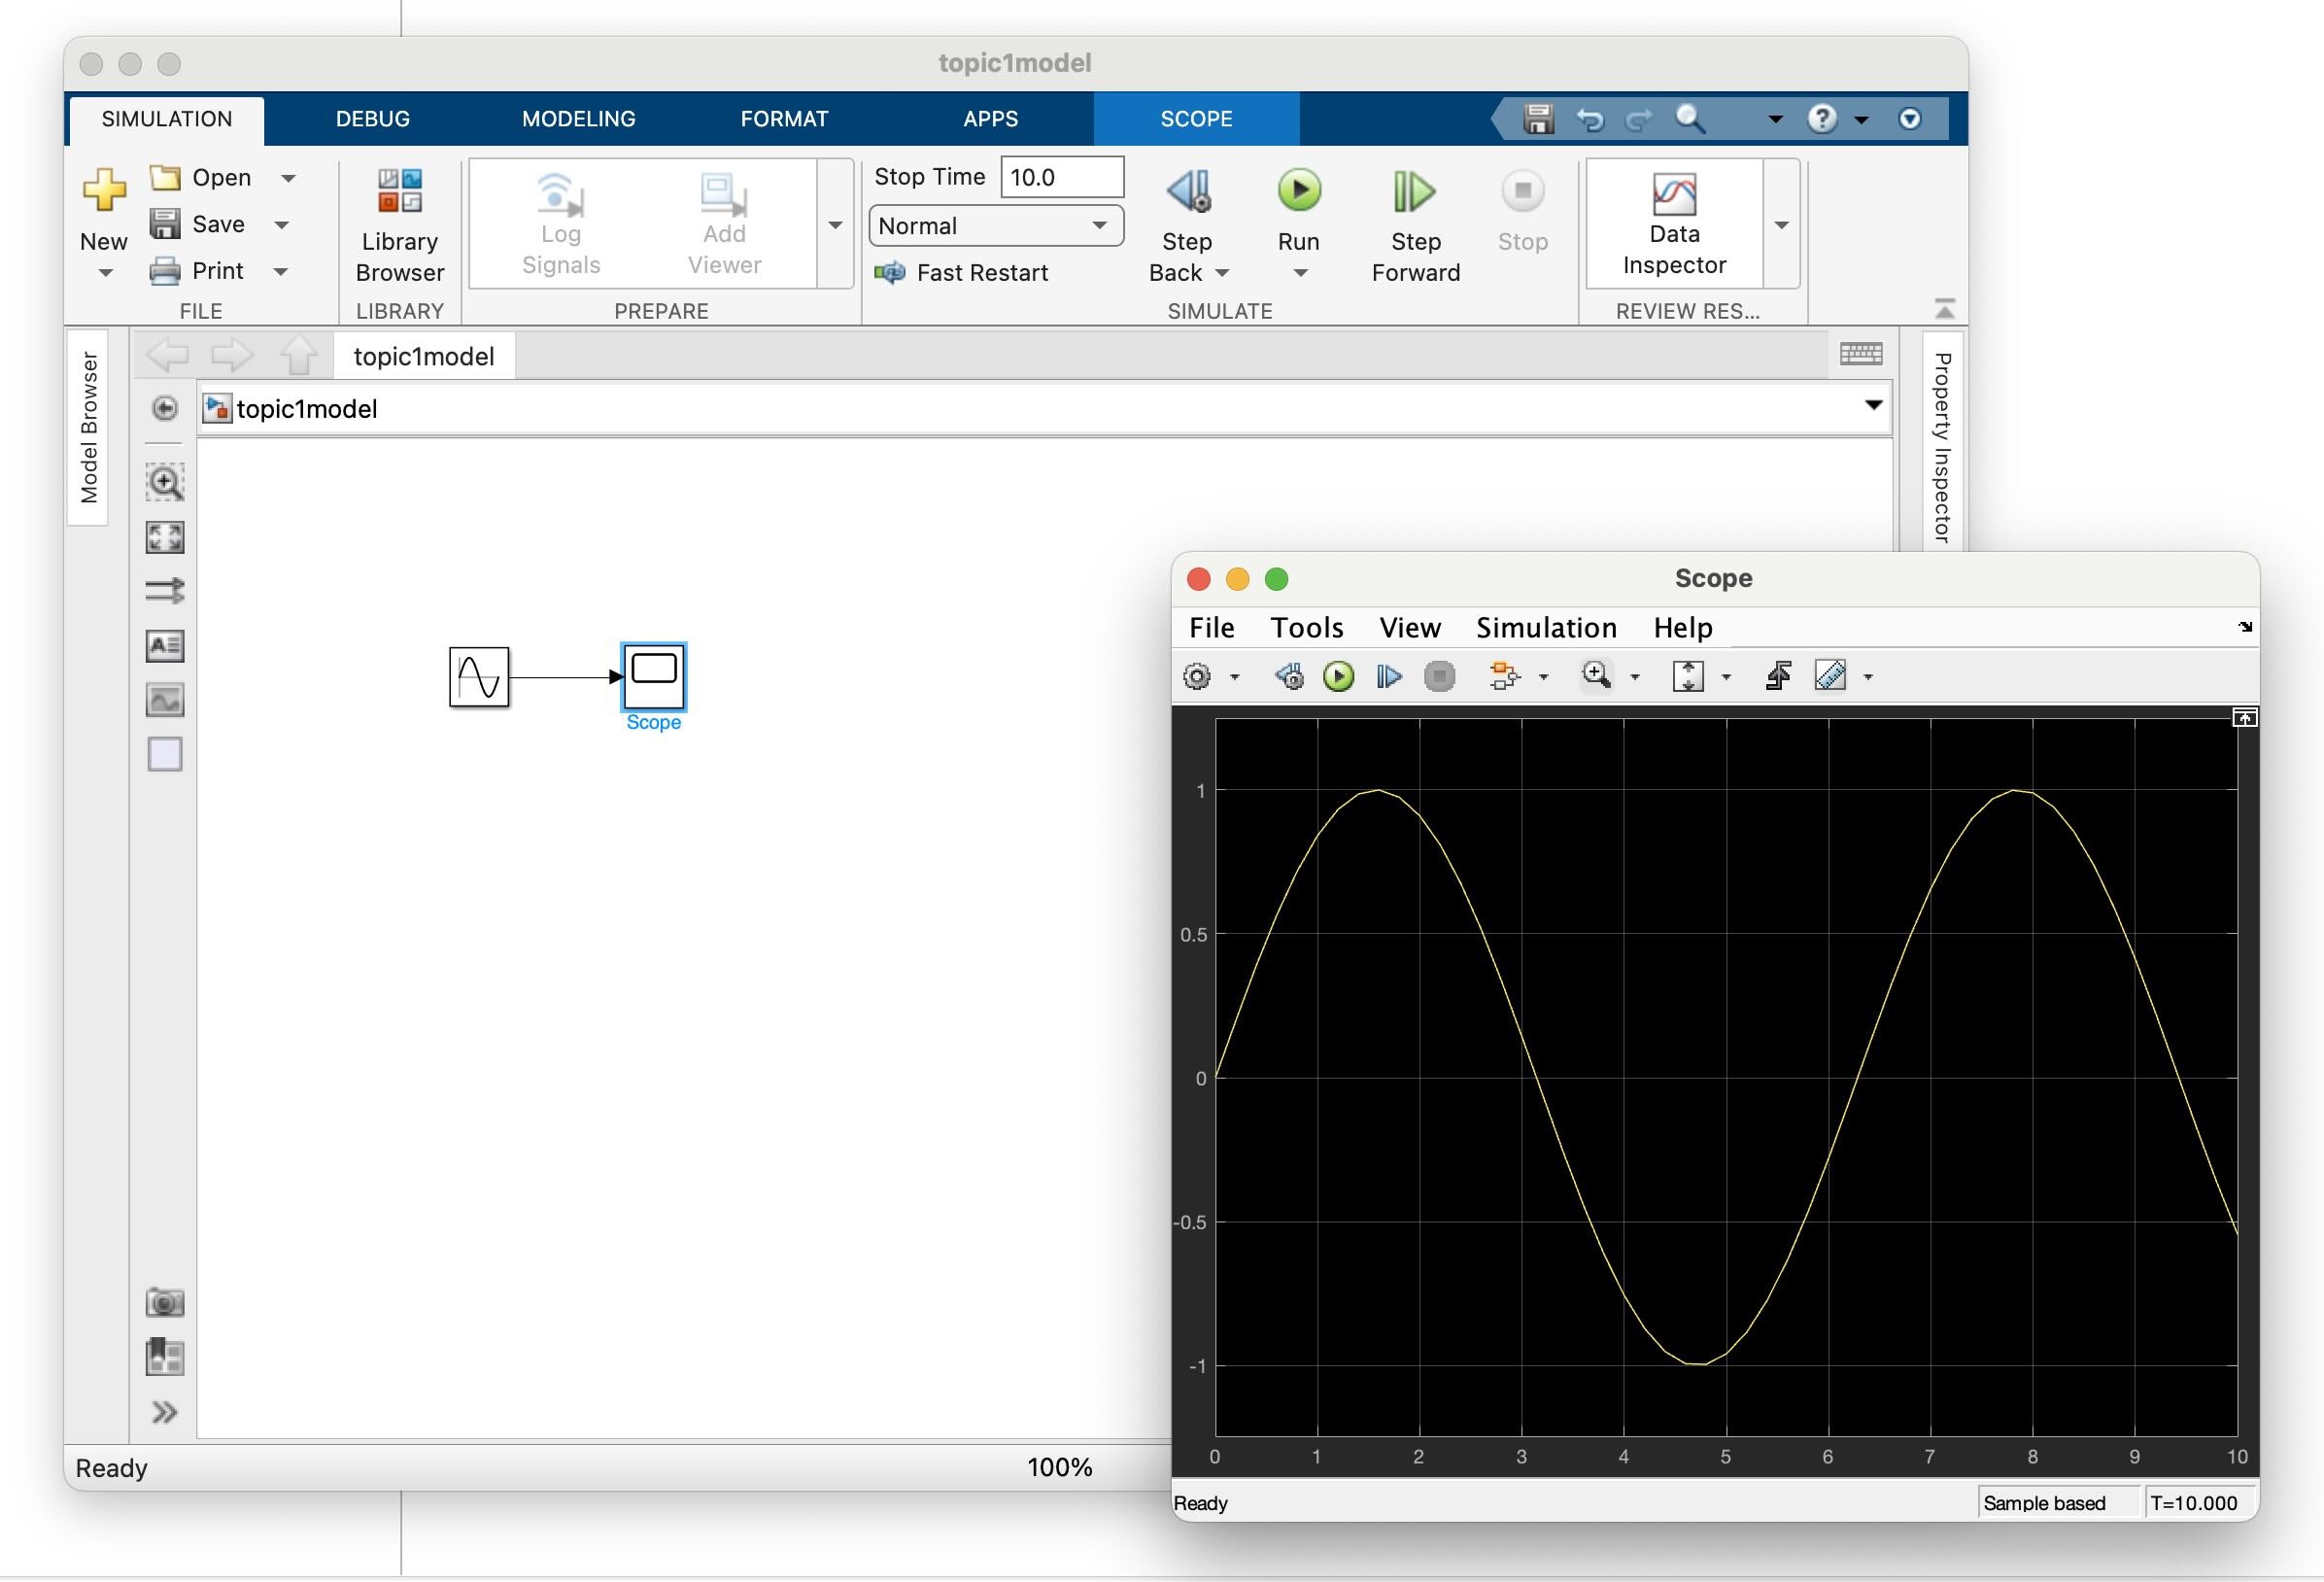
\includegraphics[height=0.6\textheight]{topic1img1}

\end{frame}

\begin{frame}
\frametitle{Setting up variables}
\begin{itemize}
\item
Double click the Sine block and change the amplitude to \CODE{AA} and the frequency to \CODE{ww}
\item
Because these variables aren't (yet) defined in Matlab you'll see some red warning `glow'
\item
Create a new m-file called something like \texttt{topic1run.m} and define them:
\end{itemize}
\includematlab{workshop1.m}{slx}
\begin{itemize}
\item
If you run this file, it will automatically run the Simulink model
\item
Now we want to get data out of the model, too
\item
More than one way to do this, simplest is with \Mbutton{To workspace} block
\end{itemize}

\end{frame}

\begin{frame}
\frametitle{Logging data from Simulink}
\centering
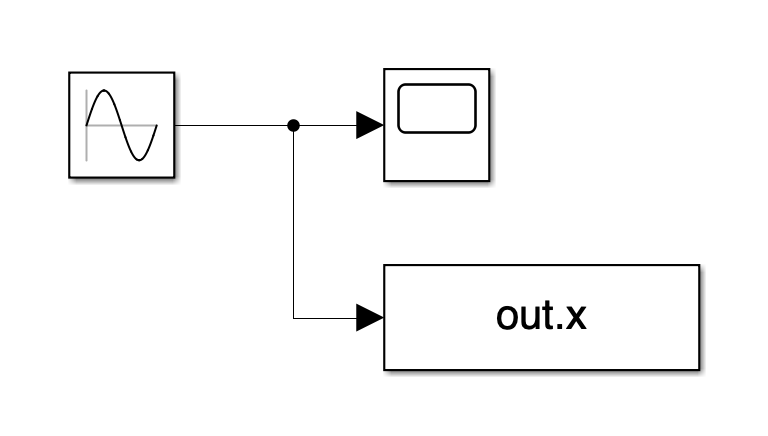
\includegraphics[width=0.5\textwidth]{topic1img_simout}
\begin{itemize}
\item
Double click the \Mbutton{To workspace} block to change its variable name to \CODE{x}
\item
Below your \CODE{sim()} command, add:
\end{itemize}
\includematlab{workshop1.m}{slx2}
\begin{itemize}
\item
Add a new variable \CODE{tmax = 20;} and figure out how to parameterise this in the Simulink model
\item
You can now set up a model in Simulink and produce results
\end{itemize}

\end{frame}

\SUBCONCEPT{Simulink modelling}

\begin{frame}
\frametitle{Dynamic model in Simulink}
There are lots of ways of creating dynamic models in Simulink, we start with the barest of basics:
\[
   \sum F = m\,\ddot x = - c\,\dot x - k\,x + f
\]
You'll need the following blocks:
\begin{itemize}
\item \Mbutton{Step}, \Mbutton{Sum}, \Mbutton{Gain}, \Mbutton{Integrator}, \Mbutton{To workspace}
\item Double click the \Mbutton{Sum} to change it to be rectangular and have three inputs defined \CODE{+--}
\item Rotate blocks with CTRL+R on Windows or CMD+R on Mac
\end{itemize}

\centering
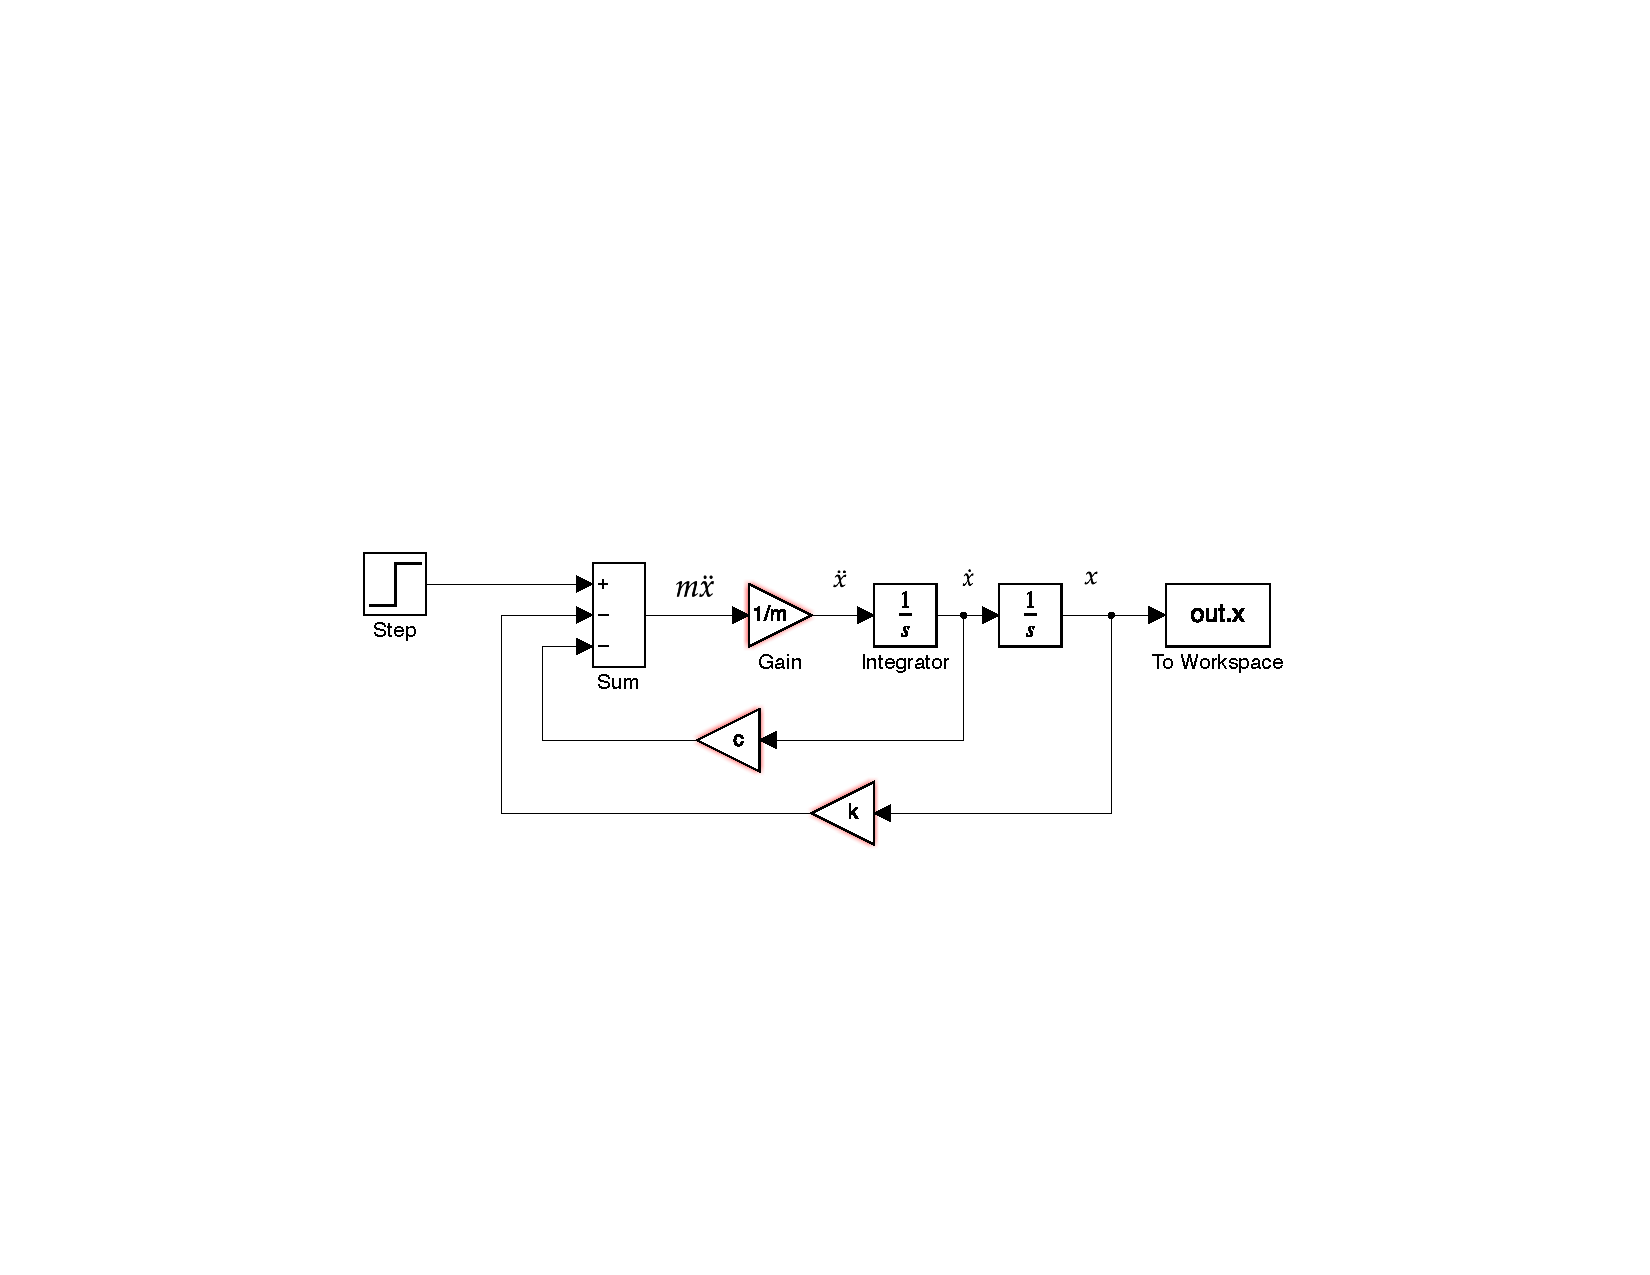
\includegraphics[width=0.8\linewidth]{topic1_sim_msd.pdf}

\end{frame}

\begin{frame}
\frametitle{Dynamic model results}
\begin{itemize}
\item Save that Simulink model as \texttt{topic1msd.slx}
\item Create a matching m-file \texttt{topic1run.m}:
\end{itemize}
\includematlab{workshop1.m}{slx3}
\begin{itemize}
\item Results shown over the page
\end{itemize}
\end{frame}

\begin{frame}
\frametitle{Dynamic model results}
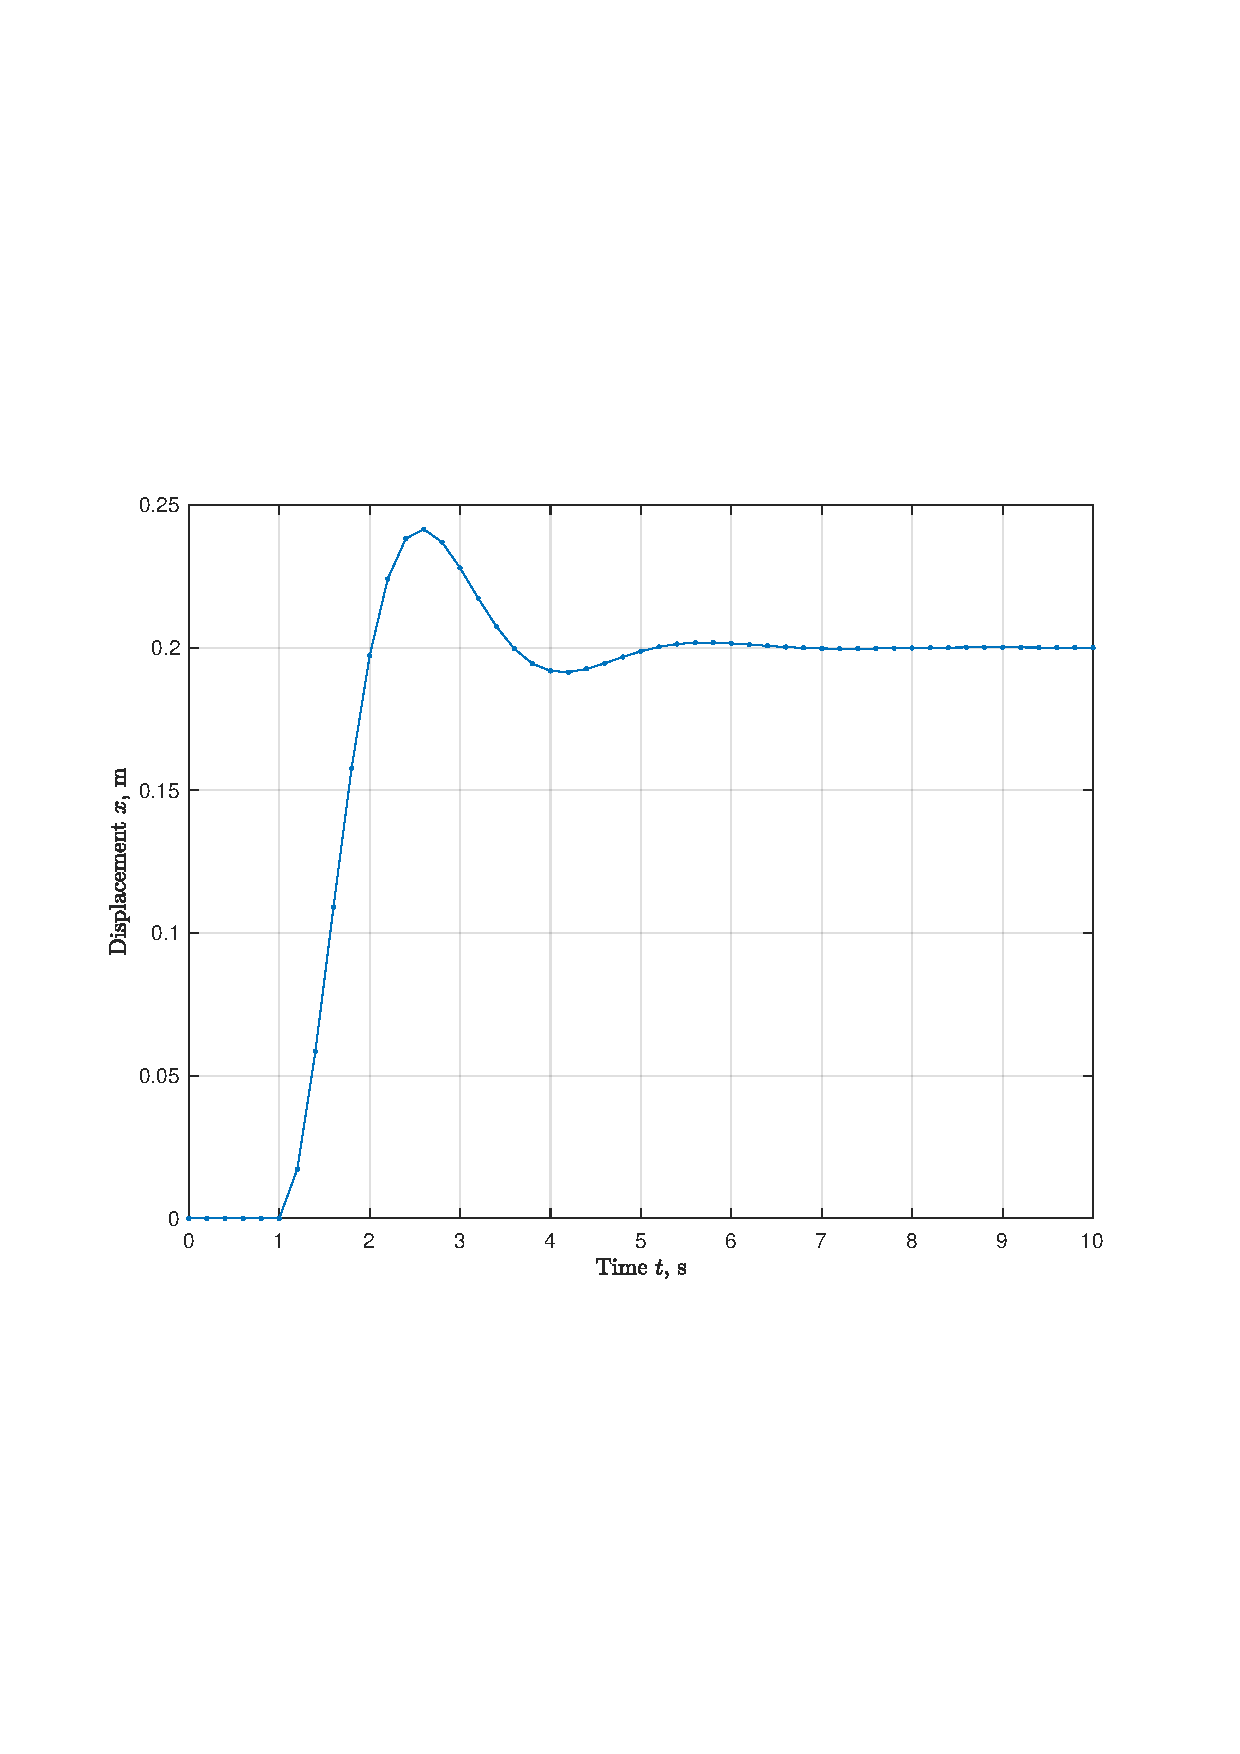
\includegraphics[width=\linewidth,trim=0 200 0 200,clip]{topic1_msd_step.pdf}
\end{frame}

\begin{frame}
\frametitle{Final Simulink comments}
\begin{itemize}
\item Internally Simulink is using the Matlab \CODE{ode45} solver (by default) --- but it's much easier to set up complex models with block diagrams like this
\item Go to tab \Mbutton{Modeling} and click button \Mbutton{Model Settings} to improve fidelity
\item E.g., \Mbutton{Solver details} > \Mbutton{Relative tolerance} = \texttt{1e6}\\
      (yes, this can be parameterised too)
\item Note the default step response starts at $t=1$ seconds --- nonstandard
\end{itemize}
\end{frame}

\SUMMARYFRAME

\end{document}
